
The authors provided us with three graphs in order to test our
different implementations of the Tutte method.\\

These graphs have the following characteristics :

\begin{center}
\begin{tabular}{|c|c|c|}
\hline
Graph & number of vertices & number of edges \\
\hline
aiir\_traffic & 14693 & 63403\\
imdb & 9488 & 33942\\
migration & 14318 & 49460\\
\hline
\end{tabular}
\end{center}


For the first implementation with a basic structure to
work on the graph, we obtain these results~:

\begin{center}
\begin{tabular}{|c|c|c|c|}
\hline
Graph & number of iterations & mean time of execution of Tutte's algorithm & standard deviation\\
\hline
aiir\_traffic & 61 & 0.2526 & 0\\
imdb & 473 & 1.2957 & 0\\
migration & 5 & 0.006314 & 0\\
\hline

\end{tabular}
%\caption{title}
\end{center}

The results we get here is not what we expected. Despite the fact that the computation time is quite improved, the graph provided has some fixed nodes inside the grid, consequently, after the call of our implementation of the Tutte Algorithm, some edge crossing (due to those fixed nodes) appear and remove the planarity of the graph. As an explanation, we can say that by moving nodes around an internal fixed node, and in relation with the number of edges in one direction, mobile nodes tend to orient themselves to the direction of the fixed node having most of edges. With this orientation, a mobile node which is opposite to the side with a lot of edges will move to this side and create an edge-crossing.

Here are some pictures to recap:

\begin{figure}[!h]
\centering
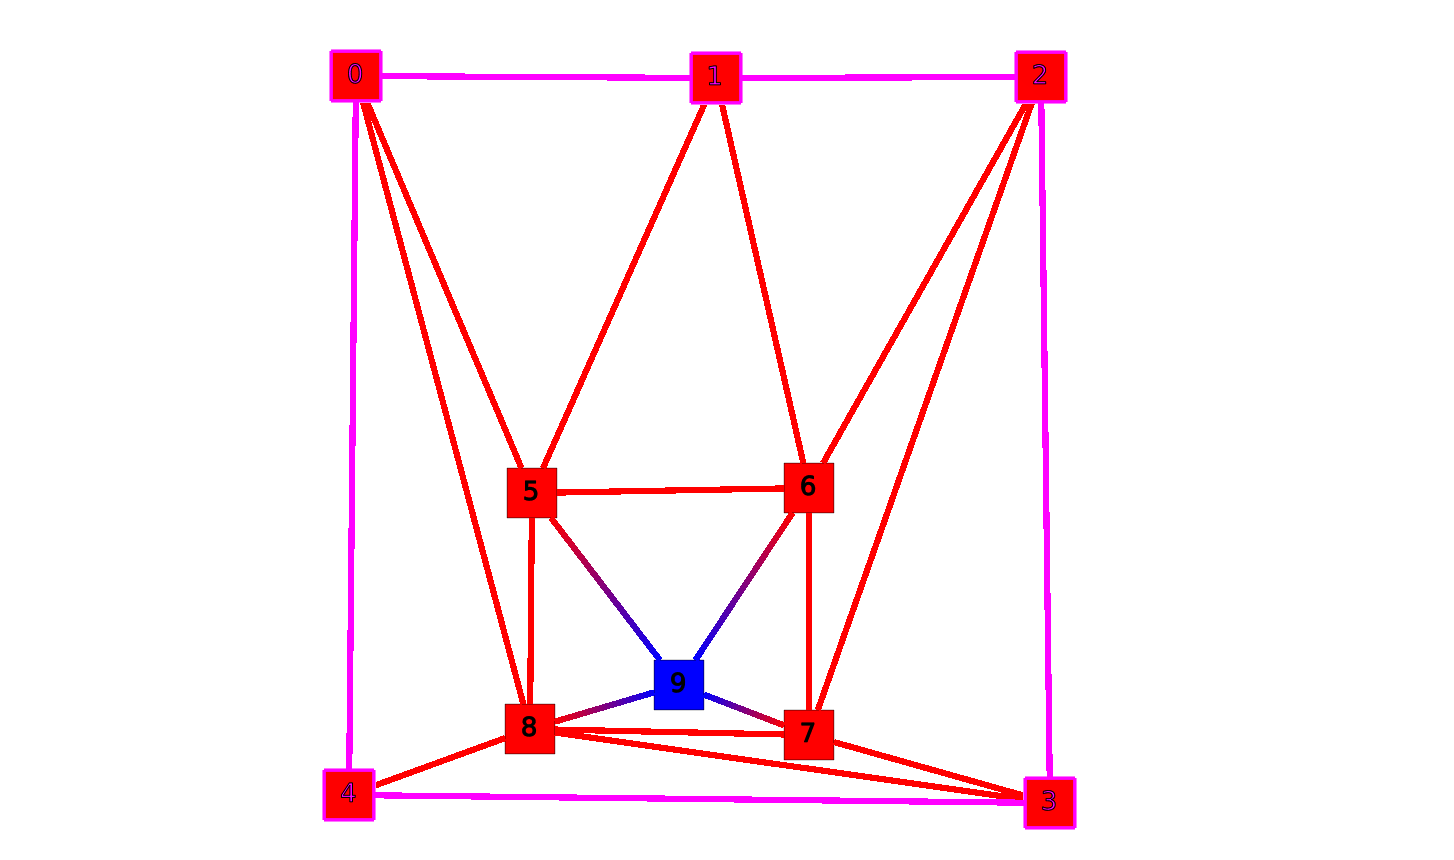
\includegraphics[scale=0.5]{snapshots/constate_fix_init.png}
\caption{One initial set}
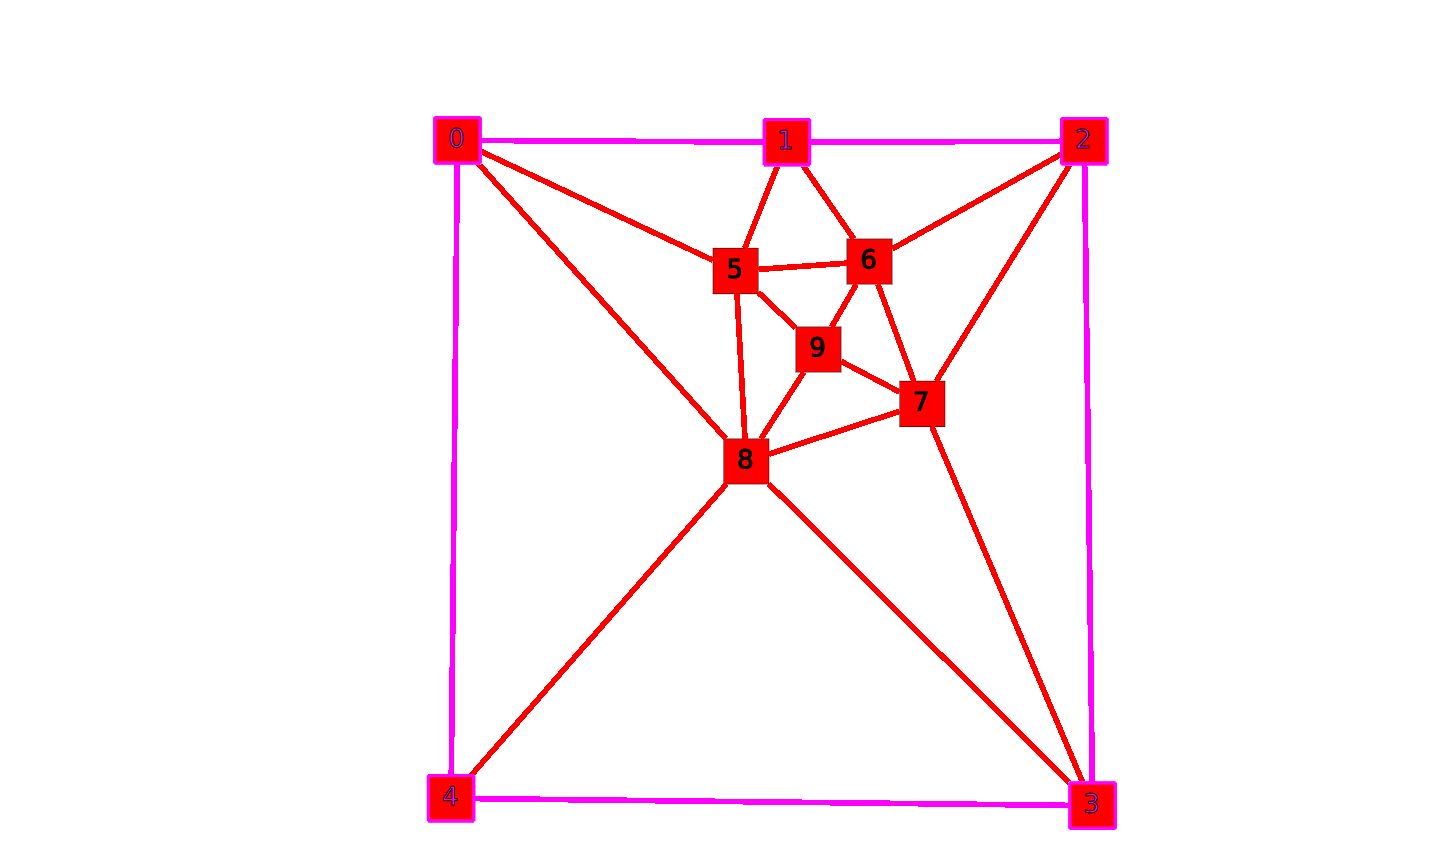
\includegraphics[scale=0.5]{snapshots/constate_nikel.png}
\caption{The set correctly modified(all nodes mobiles)}
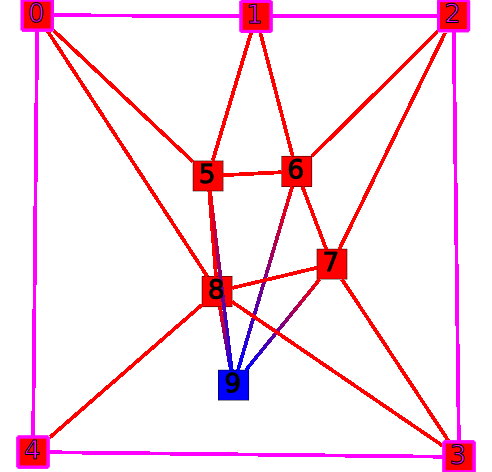
\includegraphics[scale=0.5]{snapshots/constate_probleme.png}
\caption{The set not correctly modified(one fixed node)}
\end{figure}
